\section{Perception of sound}

\subsection{Range of human hearing}
\bi

\i The frequency range of human hearing is roughly
20~Hz to 20~kHz.
This is a factor of $1000$ or roughly 10 octaves
($2^{10} = 1024$) in frequency.

\i The pressure variation range of human hearing at 1000~Hz is
roughly $2\times 10^{-5}~{\rm Pa}$ (threshold of hearing)
to $20~{\rm Pa}$ (threshold of pain).
This is a factor of $10^6$ in pressure variation or $10^{12}$
in intensity (${\rm Watt/m}^2$).

\i Compared to standard atmospheric pressure $P_{\rm atm} = 100~{\rm kPa}$,
these values are only $2\times 10^{-10}$ and
$2\times 10^{-4}$ of atmospheric pressure, respectively.
So even at the threshold of pain, the pressure change is only a few 
parts in $10^4$ of atmospheric pressure!

\i In contrast, the frequency range for human vision is
only a factor of 2 (so 1 octave);
and the intensity range of human vision is only a factor of
$10^5$ (versus $10^{12}$ for human hearing).
Thus, the human ear is a much more sensitive device than the
human eye!

\ei
%%%%%%%%%%%%%%%%%%%%%%%%%%%%%%%%%%%%%%%%%%%%%%%%
\subsection{Fechner's law and logarithms}
\bi

\i G.~T. Fechner in ``Elements of psychophysics" ($\sim 1860$):
``As stimuli are increased by multiplication, sensation
increases by addition."

\i We shall see below that Fechner's law applies
{\em approximately} to our perceptions of both the 
pitch and loudness of a sound.
(Fechner's law applies to other sensations as well, 
such as sight and smell.)

\i Mathematically, Fechner's law means that sensation is 
proportional to the {\em logarithm} of a stimulus.

\i Logarithms:
%
\be
y = \log x 
\quad\Leftrightarrow\quad
x = 10^y
\ee

The above definition is for a base-10 logarithm,
$\log x = \log_{10}x$.

\i Logarithms can be defined for arbitrary bases---for example,
base-2 logarithms, $\log_2 x$, or {\em natural} logarithms,
$\ln x = \log_e x$, whose base is $e=2.7183\cdots$.
(We will work only with base-10 logarithms in this course.)

\i Since 
%
\be
10=10^1\,,\quad
100=10^2\,,\quad
1,000,000=10^6\,,\quad
1=10^0\,,\quad
0.001=10^{-3}
\ee
%
it follows that
%
\be
\log 10=1\,,\quad
\log 100=2\,,\quad
\log 1,000,000=6\,,\quad
\log 1=0\,,\quad
\log 0.001=-3
\ee
%
Thus,
%
\be
\log 10^n = n
\ee
%
which means that each multiplicative factor of 10 increase 
in $x$ corresponds to an additive increase of $y=\log x$ by 1. 
(See Figure~\ref{f:linear-log}.)
%
\begin{figure}[htbp]
\begin{center}
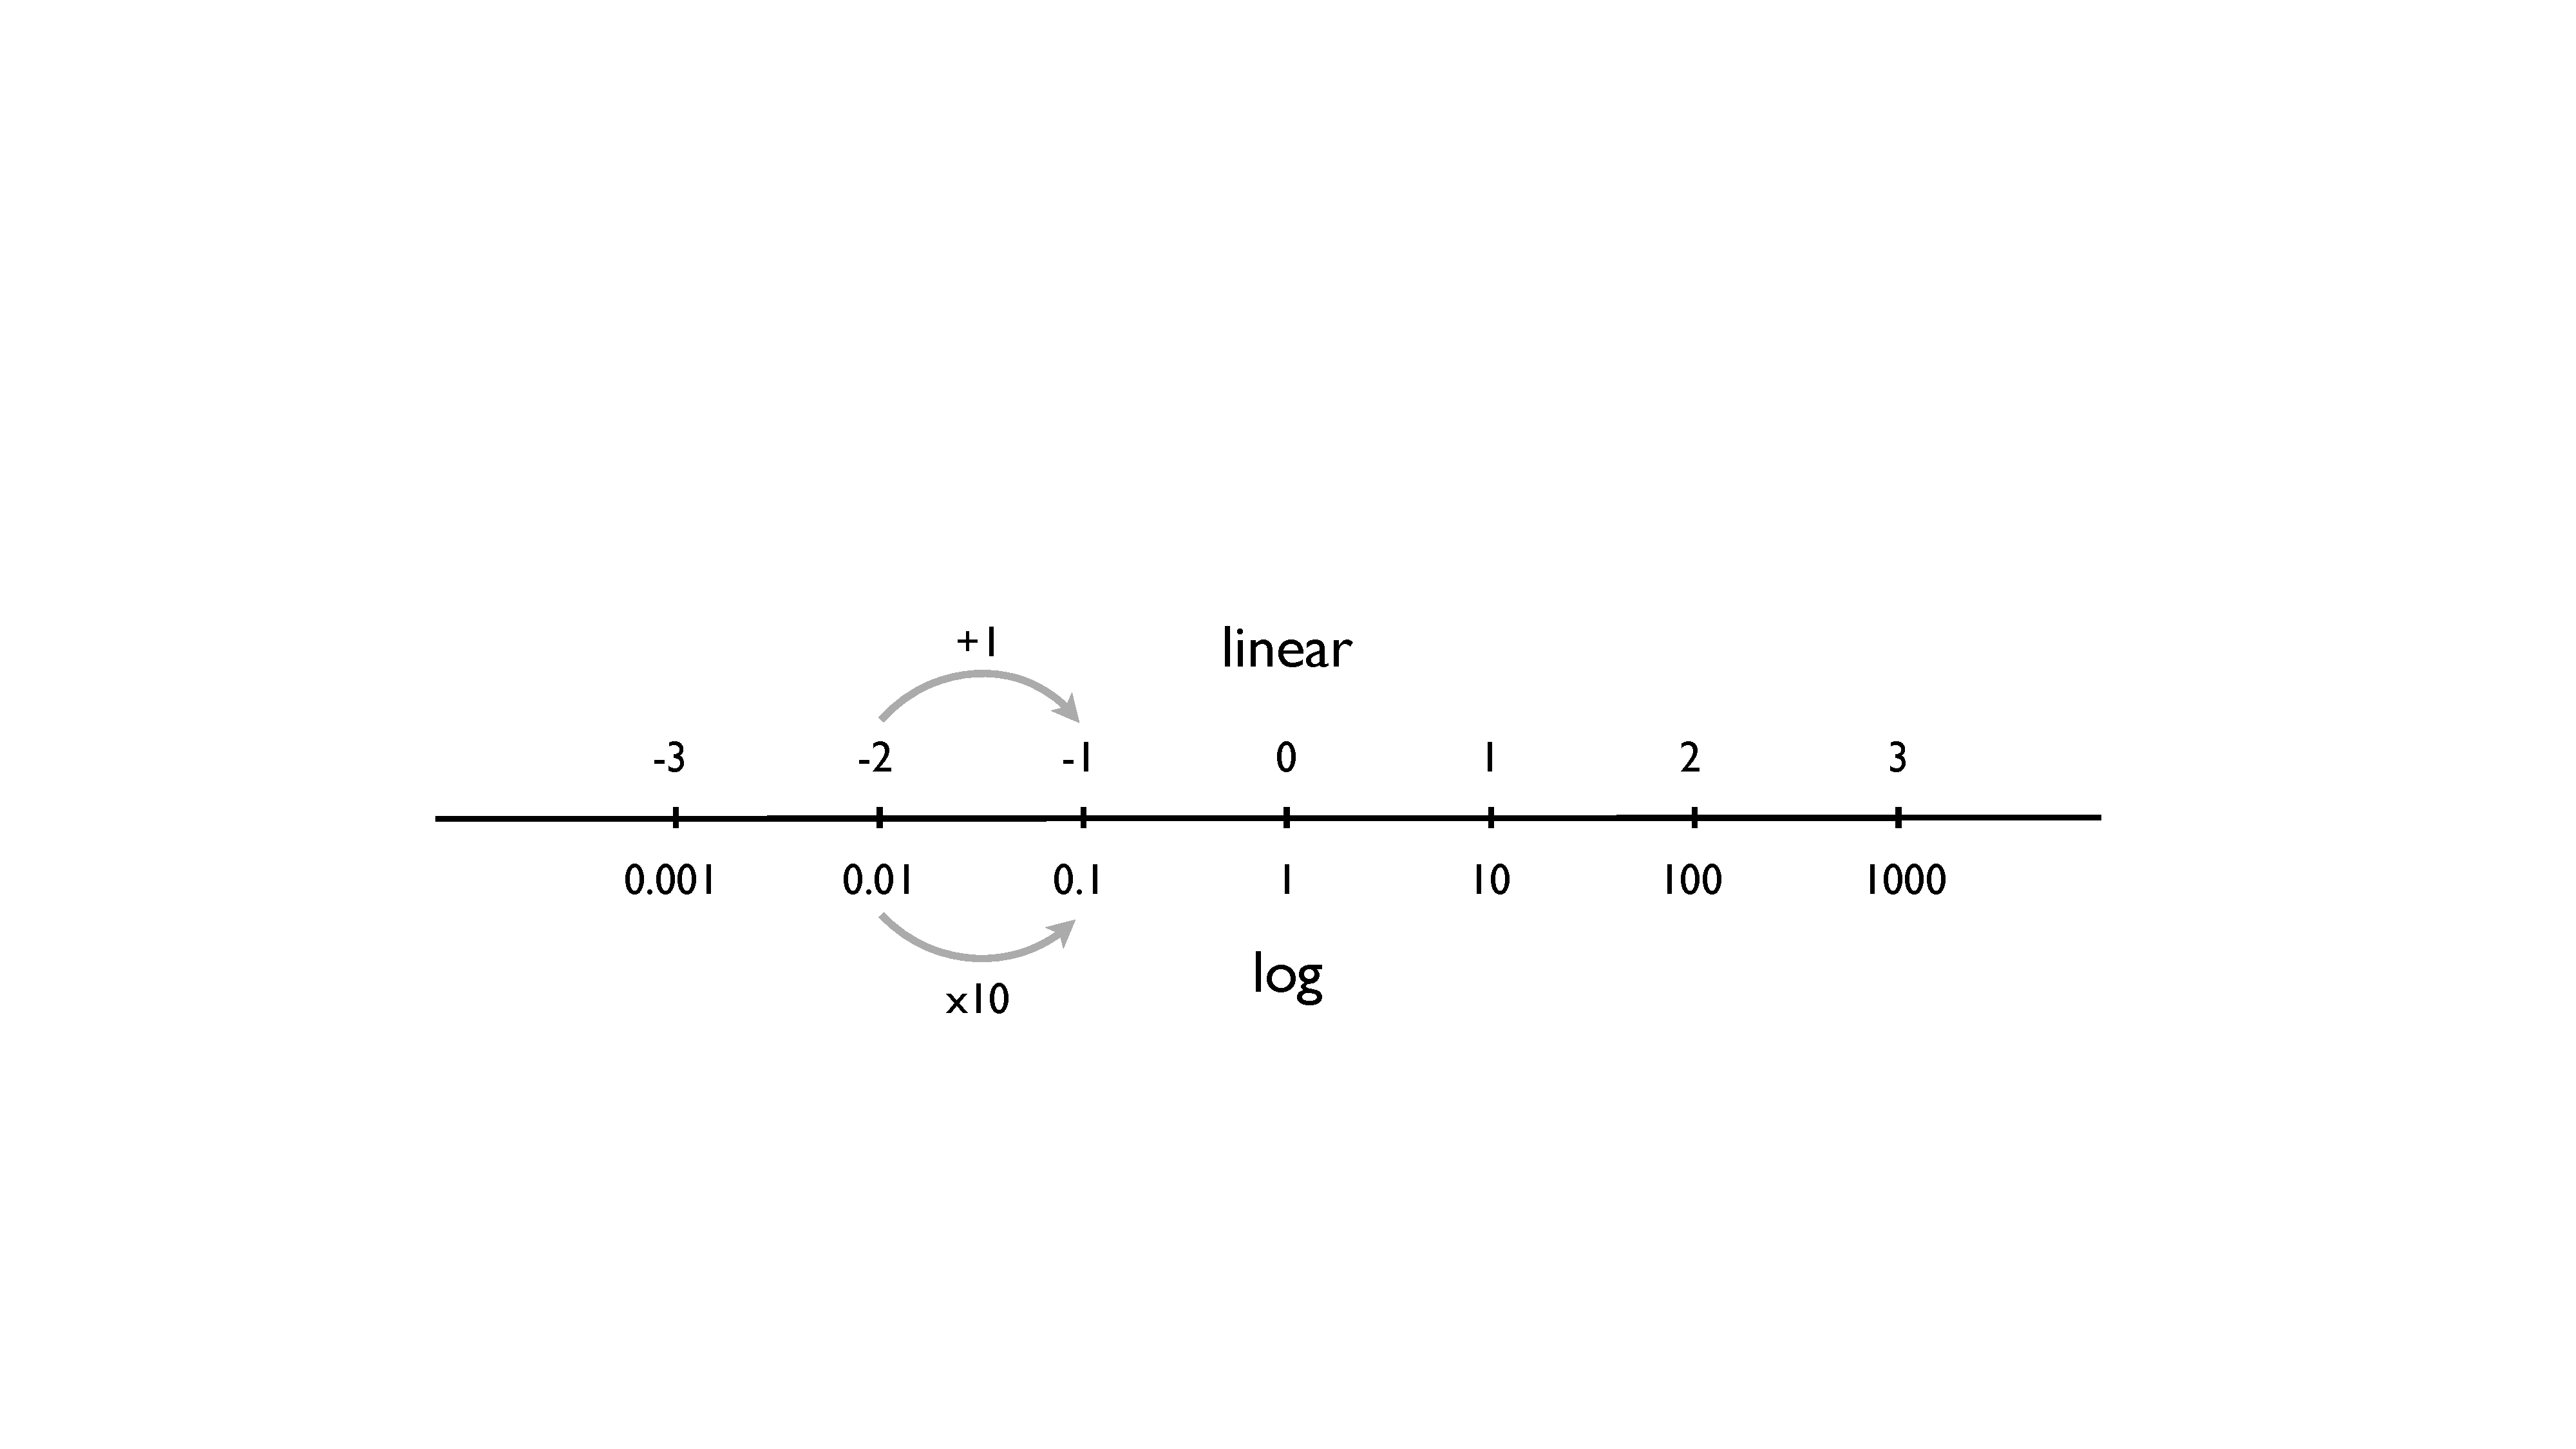
\includegraphics[width=.8\textwidth]{linear-log}
\caption{Difference between linear and logarithmic scales.
The tick marks on a linear scale are separated by a
constant additive term (here $+1$);
the tick marks on a logarithmic scale are separated by a
constant multiplicative factor (here $\times 10$).}
\label{f:linear-log}
\end{center}
\end{figure}
%

\i Key property of logarithms:
%
\be
\log(ab) = \log a + \log b\,,
\ee
%

\i \underline{Proof:}
%
\be
\log(x_1 x_2) = \log\left(10^{y_1} 10^{y_2}\right)
= \log\left(10^{y_1+y_2}\right)
= y_1 + y_2
=\log x_1 + \log x_2
\ee

\i Recall that addition of musical intervals 
corresponds to 
multiplication of the corresponding frequeny ratios.
Hence, musical intervals can be written as logarithms
of frequency ratios.

\i For example, if $R$ denotes the ratio of two
frequencies, then
%
\begin{align}
&{\rm number\ of\ octaves}
= \frac{\log R}{\log 2}
\\
&{\rm number\ of\ semitones}
= \frac{\log R}{\log (2^{1/12})}
= 12\, \frac{\log R}{\log 2}
\\
&{\rm number\ of\ perfect\ fifths}
= \frac{\log R}{\log (3/2)}
\\
&{\rm etc.}
\end{align}

\i \exer Calculate the number of semitone intervals
that correspond to a frequency ratio of 1.5 for 
a just perfect fifth.

\i \ans
%
\be
{\rm number\ of\ semitones}
= 12\, \frac{\log 1.5}{\log 2}
= 7.0196
\ee

\i Examples of logarithmic frequency scales:
Piano keyboard, musical staff, basilar membrane of the
human ear (which we shall describe below).

\i Equal divisions on the piano keyboard 
correspond to musical notes whose frequencies are related
by the same constant multiplicative factor---e.g., 
neighboring keys are 1 semitone apart, corresponding
to a frequency ratio of $2^{1/12}=1.05946$;
13 keys on a piano keyboard are an octave apart, 
corresponding to a frequency ratio of 2.

\i Useful logarithms to remember:
%
\be
\log 2 \approx 0.3\,,\quad
\log 3 \approx 0.5\,,\quad
\log 4 \approx 0.6\,,\quad
\log 5 \approx 0.7\,,\quad
\log 10 = 1
\ee
%
Note that $\log 4 = \log(2\cdot 2) = 2\log 2$ and
$\log 5 = \log(10/2) = \log 10-\log 2$.

\ei
%%%%%%%%%%%%%%%%%%%%%%%%%%%%%%%%%%%%%%%%%%%%%%%%
\subsection{The human ear}
\bi

\i The human auditory system consists of two parts: 
(i) the peripheral auditory system made up of the ear, and
(ii) the central auditory system made of the brain and the
auditory nervous system.

\i The human ear can be divided functionally into 
three basic parts
(the outer, middle, and inner ear) as shown in 
Figure~\ref{f:human-ear-diagram}.
%
\begin{figure}[htbp]
\begin{center}
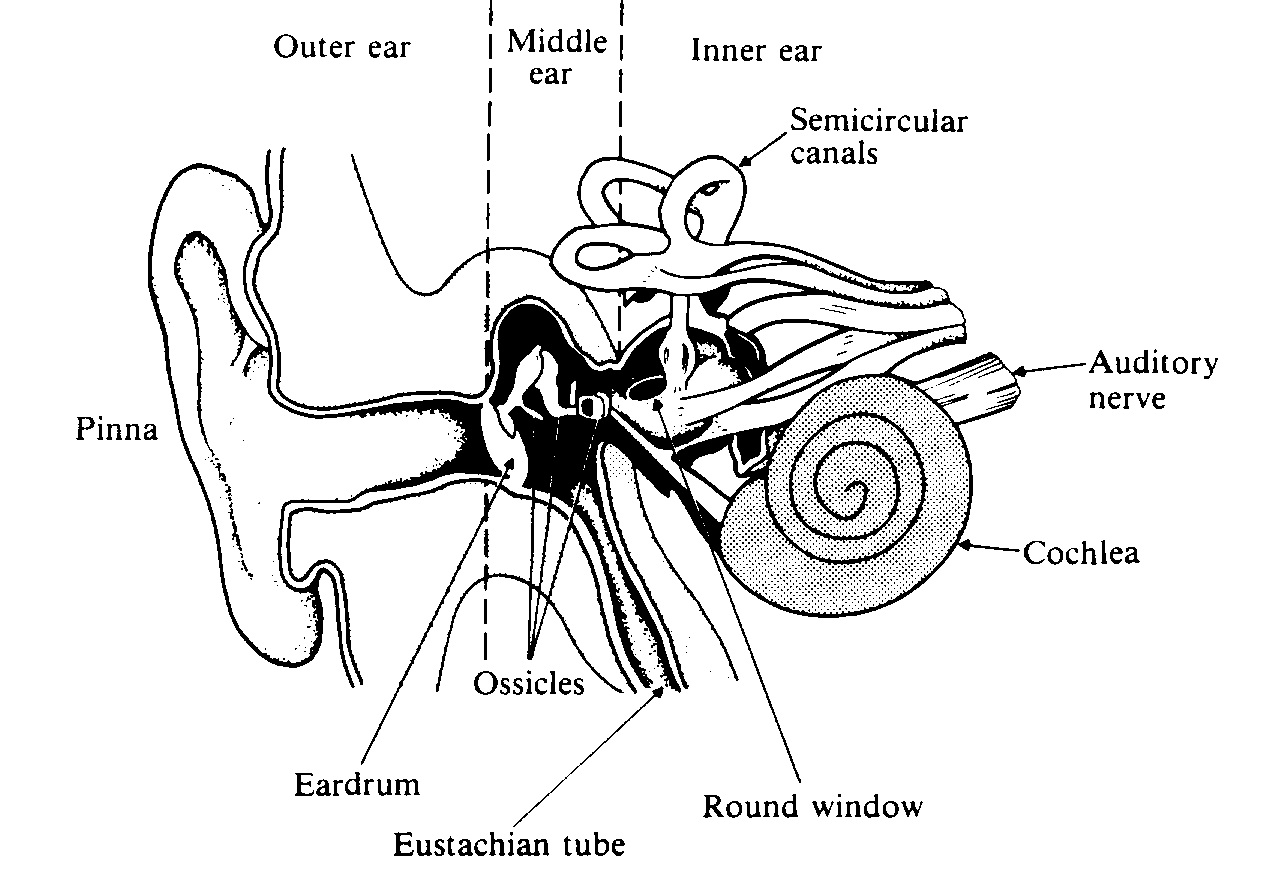
\includegraphics[width=.8\textwidth]{human-ear-diagram.jpg}
\caption{A drawing of the human ear, showing the division into
the outer, middle, and inner ear.  
Note that this drawing is not to scale.
(From ``Science of Sound" by Rossing, Moore, and Wheeler.)}
\label{f:human-ear-diagram}
\end{center}
\end{figure}
%

\i The outer ear consists of the pinna and auditory canal,
which collects the sound (i.e., pressure waves in the air)
and funnels it to the middle ear.

\i The middle ear consists of the ear drum and ossicles
(three small bones called the hammer, anvil, and stirrup,
based on their shapes).
The pressure wave at the ear drum is amplified ($\sim 30\times$) 
by the ossicles as it is transmitted to the oval window.
 
\i The inner ear consists of the semi-circular canals,
which are responsible for balance, and the 
cochlea, which is responsible for converting the mechanical
sound waves to electrical impulses that get sent to the
brain via the auditory nerve.

\i A schematic representation of the ear is shown in
Figure~\ref{f:human-ear-schematic}.
%
\begin{figure}[htbp]
\begin{center}
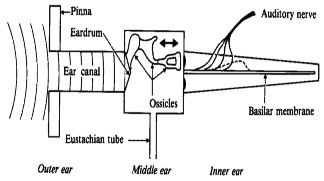
\includegraphics[width=.8\textwidth]{human-ear-schematic.jpg}
\caption{A schematic representation of the human ear, with an
uncoiled cochlea.
(From ``Science of Sound" by Rossing, Moore, and Wheeler.)}
\label{f:human-ear-schematic}
\end{center}
\end{figure}
%

\i In Figure~\ref{f:human-ear-schematic}, the cochlea is unwound.
The length of an unwound cochlea is approximately 3.5~cm (so a 
little less than 1.5~inches).
The basilar membrane divides the cochlear tube into two sections
called the {\em scala vestibuli} at the top of the diagram, 
and the {\em scala tympani} at the bottom.
The ossicle bones are, from left to right, 
the hammer, anvil, and stirrup.

\i Figure~\ref{f:cochlea-uncoiled} is a schematic
representation of an unwound cochlea.
%
\begin{figure}[htbp]
\begin{center}
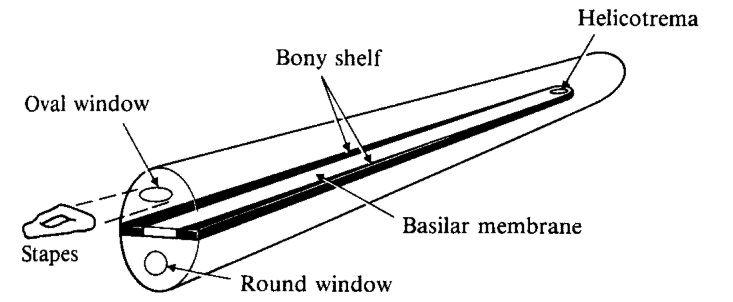
\includegraphics[width=.8\textwidth]{cochlea-uncoiled.jpg}
\caption{A schematic representation of an unwound cochlea.
The region above the basilar membrane is called the {\em scala vestibuli};
the region below the basilar membrane is called the {\em scala tympani}.
The helicotrema is a hole in the basilar membrane connecting
the two sections of the cochlea. 
(From ``Science of Sound" by Rossing, Moore, and Wheeler.)}
\label{f:cochlea-uncoiled}
\end{center}
\end{figure}
%

\i The organ of Corti rests on the basilar membrane.
It contains rows of tiny hair cells that are connected to
the auditory nerve fibers.

\i Each hair cells has many hairs, called {\em stereocilia},
which bend in response to motions of the basilar membrane.
The bending of the stereocilia stimulate the hair cells,
which trigger the auditory nerve fibers to send electrical
impulses to the brain.

\i When the stapes (stirrups) press against the oval window,
a pressure wave is set up in the cochlear fluid, causing
the basilar membrane to have ripples as shown in 
Figure~\ref{f:cochlea-uncoiled-schematic}.
%
\begin{figure}[htbp]
\begin{center}

\includegraphics[width=.8\textwidth]{cochlea-uncoiled-schematic.png}
\caption{A schematic representation showing the effects of
a pressure wave propagating through the cochlear fluid.
OW stands for oval window; RW for round window;
SV for scala vestibuli; ST for scala tympani; and
H for helicotrema.
The location of maximum displacement of the basilar membrane
(BM) depends on the frequency of the sound.
(From {\tt commons.wikimedia.org}.)}
\label{f:cochlea-uncoiled-schematic}
\end{center}
\end{figure}
%

\i The location of maximum displacement of the basilar 
membrane depends on the frequency of the incident sound wave:
{\em High-frequency} sound waves produce maximum displacements 
of the basilar membrane {\em closer} to the stirrups;
{low-frequency} sound waves produce maximum displacements 
of the basilar membrane {\em further} from the stirrups.

\i A pure tone (i.e., a single frequency sound wave)
excites a relatively wide region (1.3~mm, having 
approximately 1300~neurons) of the basilar membrane.
This region is called a {\em critical band}.

\i There are 24 critical bands on the basilar membrane
that span the audible frequency range from $20$ to $\approx 20~$kHz.

\i The center frequencies of the critical bands are spaced 
logarithmically along the basilar membrane, similar to 
the frequencies of the keys on a piano keyboard.
In other words, equal distances along the basilar membrane 
correspond to equal ratios of the central frequencies as shown
in Figure~\ref{f:basilar-resonance-max}.
%
\begin{figure}[htbp]
\begin{center}
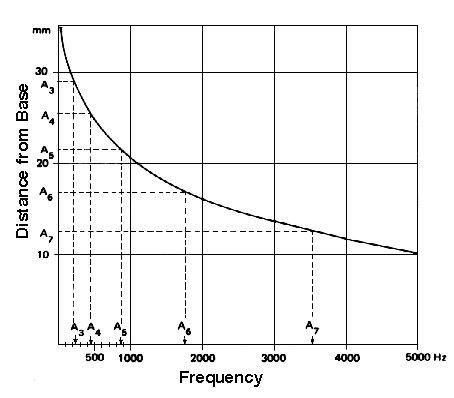
\includegraphics[width=.6\textwidth]{basilar-resonance-max.jpg}
\caption{Position of the maximum displacement on 
the basilar membrane as a function of the pure tone 
frequency.
(From ``Science of Sound" by Rossing, Moore, and Wheeler.)}
\label{f:basilar-resonance-max}
\end{center}
\end{figure}
%

\i Thus, the location of maximum displacement of the 
basilar membrane has a {\em logarithmic frequency response},
in agreement with Fechner's law.

\i The bandwidths of the critical bands are approximately
constant ($\approx 100$~Hz) for frequencies below about 500~Hz;
at higher frequencies, the bandwidths increase in proportion 
to the center frequencies, having values slightly less than 
one-third of an octave (or a major third) about each center
frequency.

\i The fact that the human ear acts like a spectrum analyser 
for sound waves (with different parts of the basilar membrane
repsonding to different frequency sound waves) 
is called the {\em place theory of pitch}.

\i Sound waves can enter the inner ear via {\em air conduction} 
as discussed above.
They can also enter the inner ear via {\em bone conduction} through 
the skull.

\i Humming is an example of a sound that is heard mostly 
via bone conduction.
By plugging your ears with your fingers when humming 
(thus blocking the air path), the humming can actually sound louder.

\i Hearing through bone conduction is the reason why our
voices sound different when we hear ourselves speak on a tape recorder.
The microphone of a tape recorder picks up our voice as it 
is heard via air conduction.
But we hear our own voice partly via air conduction and partly via
bone conduction.

\ei
%%%%%%%%%%%%%%%%%%%%%%%%%%%%%%%%%%%%%%%%%%%%%%%
\subsection{Binaural hearing}
\bi

\i The fact that we have two ears allows us to better 
locate the source of a sound (similar to depth perception
using two eyes---i.e., binocular vision).
 
\i For frequencies above about 4000~Hz, localization is
accomplished via an {\em intensity} difference of the 
sound reaching the two ears.
At these higher frequencies, sound does not easily 
diffract around the head, so one ear is effectively in
the ``shadow" of the head and receives less intense sound.
The brain interprets the ear that hears the less 
intense sound as being further from the source of sound.

\i For frequencies below about 1000~Hz, localization is
accomplished via a difference in the {\em time of arrival}
(or, equivalently, a phase difference) of the sound 
reaching the two ears.
The brain interprets the ear that hears the time-delayed 
sound as being further from the source of the sound.

\ei
%%%%%%%%%%%%%%%%%%%%%%%%%%%%%%%%%%%%%%%%%%%%%%%
\subsection{Loudness}
\bi

\i Loudness is our perception of the relative 
strength of a sound.
It depends on the amplitude of the sound wave,
its frequency, and its duration.
(Here we will concentrate on the loudness of 
pure tones; in a later subsection we will discuss
the complications associated with the loudness of 
complex tones.)

\i Loudness is a {\em relative} quantity in 
the sense that it involves a comparison between 
two different sounds---e.g., we say that this 
sound is twice as loud as that one.
In many of the formulae below, we will take our 
reference sound to be at the threshold of hearing.

\i As we shall describe in more detail below,
the human ear is most sensitive to sounds
with frequencies around 4000~Hz.
For example, a sound wave with a frequency of
100~Hz is perceived to be quieter than 
a sound wave with the same amplitude, 
but with a frequency of 4000~Hz.
%(See Figure~\ref{f:equal-loudness}.)

\i Sounds with durations less than about a half
a second are perceived to be quieter than the 
same sound having a duration of about a second.

\i The loudness of a sound that has 
a duration greater than several tens of seconds 
is perceived to {\em decrease} slightly over time.

\i This is due to {\em sensory adaptation} of
the brain.
A long-duration stimulus is increasingly ignored
by the brain as it realizes that there is no 
associated danger.
The firing rate of neurons decreases as the
duration of the stimulus increases;
the firing rate increases when there is a {\em change} 
in the stimulus.

\i Loudness depends on the {\em intensity} of
a sound wave but is not equal to it.
As we shall see below, loudness is more closely
related to the {\em logarithm} of the intensity, 
in line with Fechner's law relating stimulus 
to sensation.

\i Recall that the intensity of a wave is the
rate at which energy passes through a unit area
perpendicular to the direction of wave propagation.
The units of intensity are W/m$^2$, corresponding 
to ${\rm energy}/({\rm area}\cdot{\rm time})$.

\i The intensity $I$ of a sound wave is related to 
the pressure difference $p$ via
%
\be
I= \frac{p^2}{\rho v}
\label{e:Ivsrho2}
\ee
%
where $\rho$ is the density of air and $v$ is the speed 
of sound.
Thus, the intensity is proportional to the 
{\em squared amplitude} of the wave.

\i The {\em sound intensity level} 
(sometimes denoted $SIL$) is defined as
%
\be
L_I = \log(I/I_0)\ {\rm bels}
= 10\log(I/I_0)\ {\rm dB}
\ee
%
where $I_0=10^{-12}~{\rm W}/{\rm m}^2$ is the intensity
for the threshold of hearing at $f=1000~{\rm Hz}$.

\i Note that 10~dB (decibels) equals 1 bel.
(A bel is named after Alexander Graham Bell, the inventor
of the telephone.)

\i \ex Doubling the intensity of a sound wave
corresponds to an increase in the sound intensity 
level by $10\log 2 \approx 3~{\rm dB}$.

\ex Increasing the intensity of a sound wave by
a factor of 10 corresponds to an increase in the 
sound intensity level by $10\log 10 = 10~{\rm dB}$.

\i Since our ears and sound level meters actually
measure pressure differences away from atmospheric
pressure, it is often more convenient to work with
{\em sound pressure level} (sometimes denoted $SPL$) 
defined by:
%
\be
L_p = 20\log(p/p_0)\ {\rm dB}
\ee
%
where $p_0=2\times 10^{-5}~{\rm Pa}$ is the 
pressure difference 
for the threshold of hearing at $f=1000~{\rm Hz}$.

\i Note that 
%
\be
L_p\approx L_I
\ee
%
at ordinary temperatures and atmospheric pressures.
This follows from Equation~\ref{e:Ivsrho2}, which
relates intensity $I$ to pressure difference $p$.
($L_p$ and $L_I$ are {\em exactly} equal to one another
at $30^\circ~{\rm C}$ and $100~{\rm kPa}$, for which
$p_0^2 = I_0\rho v$.)

\i Although sound intensity level $L_I$ and sound 
pressure level $L_p$ are both 
quantative measures of the strength of a sound wave,
neither takes into account the frequency-dependence
of the response of the human ear.

\i In 1933, H.~Fletcher and W.A.~Munson experimentally 
determined {\em equal-loudness} curves for pure 
tones by carrying out tests on many people.
Their results were very similar to those shown
in Figure~\ref{f:equal-loudness}, which have been
recommended by the International Standards Organization.
%
\begin{figure}[htbp]
\begin{center}
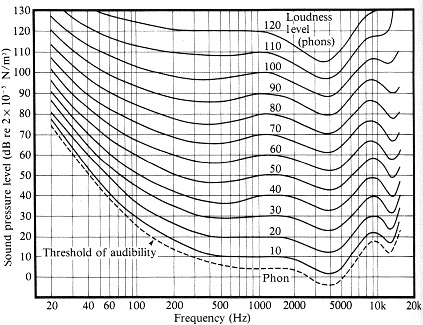
\includegraphics[width=.6\textwidth]{equal-loudness.jpg}
\caption{Equal-loudness curves (labeled in units of phons) 
for the human ear.
Note that the ear is most sensitive to frequencies around 4000~Hz.
(From ``Science of Sound" by Rossing, Moore, and Wheeler.)}
\label{f:equal-loudness}
\end{center}
\end{figure}
%

\i The equal-loudness curves are labeled by values of
constant {\em sound loudness level} $L_L$.
The units of $L_L$ are {\em phons}.
Numerically, 
%
\be
L_L\ ({\rm phon}) = L_p\ ({\rm dB})
\quad
{\rm at}\  f=1000~{\rm Hz}
\ee

\i Curves of constant phon are perceived to be 
equally-loud at different frequencies.
This means that at low frequencies (e.g., 100~Hz), 
the sound pressure
level must be substantially higher than at 
$f=1000~{\rm Hz}$ for a sound to be perceived as being
equally loud.
From the figure, we see that our ears are most sensitive 
to sounds having frequencies near $f=4000~{\rm Hz}$.

\i \exer 
What is the sound pressure level at 100~Hz for a 
sound with a sound loudness level of 40~phon?

\i \ans 
Using Figure~\ref{f:equal-loudness}, we see that
the $L_L=40~{\rm phon}$ equal-loudness curve has
$L_p=50~{\rm dB}$ at $f=100~{\rm Hz}$.

\i One can purchase a sound-level meter that will
measure the sound pressure level $L_p$, with 
different frequency responses:

The C-weighting network gives a flat frequency response,
corresponding to measurements of the standard sound 
pressure level $L_p$ in dB.

The A-weighting network has a frequency response that
falls-off at low frequencies, which mimics the sensitivity 
of the human ear.
Measurements of the sound pressure level using A-weighting, 
denoted $L_p(A)$, are in units of dBA, which can 
be thought of as a substitute for phons.

\i But even the sound loudness level $L_L$ has problems.
Although it takes into account the frequency-dependence
of the response of the human ear, the numerical values
of $L_L$ don't reflect the fact that 
{\em a factor of 10 
increase in intensity corresponds to only a factor of 
2 increase in the perceived loudness of a sound.}
(Like the equal-loudness curves, this factor of 2 
increase in the perceived loudness was determined by
testing many people.)

\i To overcome this problem, one defines the 
{\em subjective loudness level} $S$ via
%
\be
S= \, 2^{(L_L-40)/10}~{\rm sone}
\ee

\i Numerically,
%
\be S = 1~{\rm sone} 
\quad\Leftrightarrow\quad
L_L = 40~{\rm phon} 
\ (=40~{\rm dB\ at}\ f=1000~{\rm Hz})
\ee

\i Table~\ref{t:loudnesslevels} compares different 
measures of loudness.
%
\begin{table}[htbp]
\begin{center}
\begin{tabular}{|c|c|c|c|}
\hline
& $L_p\approx L_I$ (dB) at 1000 Hz & $L_L$ (phon) & $S$ (sone) \\
\hline
Threshold of hearing & 0 & 0 & 1/16 \\
Recording studio & 20 & 20 & 1/4 \\
Quiet office & 40 & 40 & 1 \\
Ordinary conversation & 60 & 60 & 4 \\
Normal piano practice & 80 & 80 & 16 \\
Piano fortissimo & 100 & 100 & 64 \\
Threshold of pain & 120 & 120 & 256 \\
\hline
\end{tabular}
\caption{Comparison of different measures of loudness.}
\label{t:loudnesslevels}
\end{center}
\end{table}

\i Figure~\ref{f:OSHA-table} is a table with the
Occupational Safety and Health Administration 
(OSHA) guidelines for noise exposure.
%
\begin{figure}[htbp]
\begin{center}
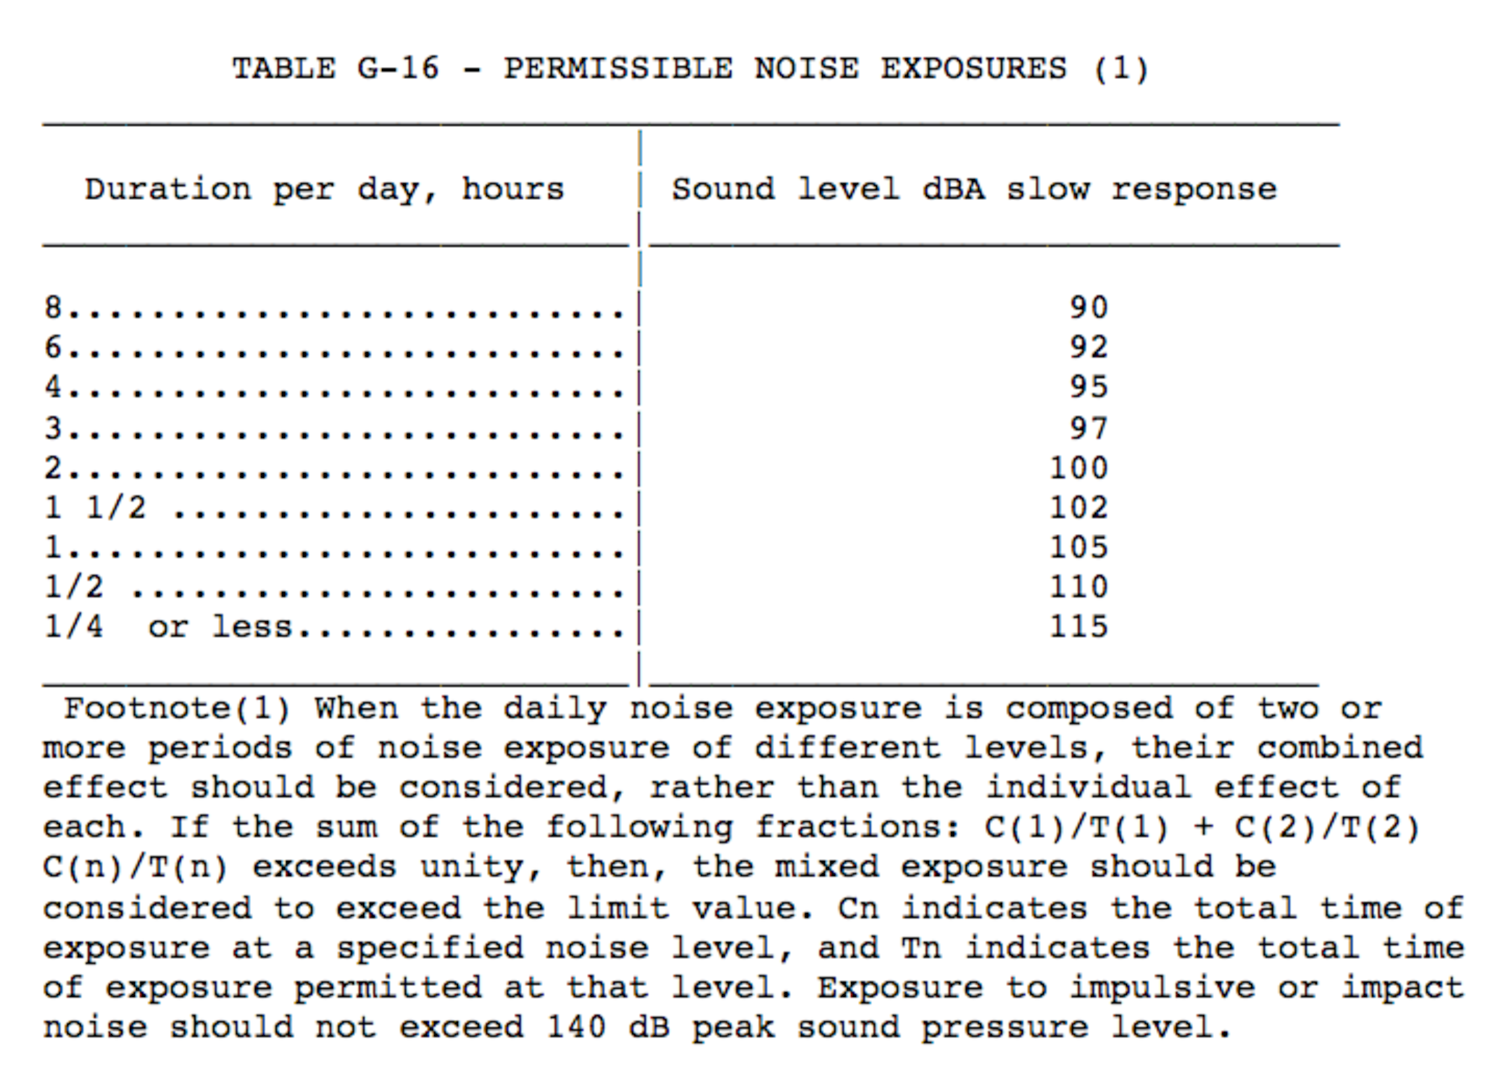
\includegraphics[width=0.8\textwidth]{OSHA-table}
\caption{OSHA permissible noise exposure levels.
(From {\tt www.osha.gov}, Standard Number: 1910.95.)}
\label{f:OSHA-table}
\end{center}
\end{figure}
%

\i The range of sound levels in a musical 
performance is called its {\em dynamic range}.

\i The dynamic range of a performance 
is typically between 10-20~dB, 
although it may as high as 40~dB.
(Remember that 10~dB corresponds to a $2\times$
increase in perceived loudness.)

\i Figure~\ref{f:loudness} has plots of the sound loudness
level $L_L$ and the subjective sound level $S$ versus 
intensity $I$ for a pure tone with frequency 1000~Hz.
Note that $L_L$ increases {\em additively} for
multiplicative increases in $I$,
which is consistent with Fechner's law.
This is {\em not} the case for $S$, 
which increases {\em multiplicatively} for 
multiplicative increases in $I$.
Thus, the subjective loudness level $S$ does not obey Fechner's law.
%
\begin{figure}[htbp]
\begin{center}
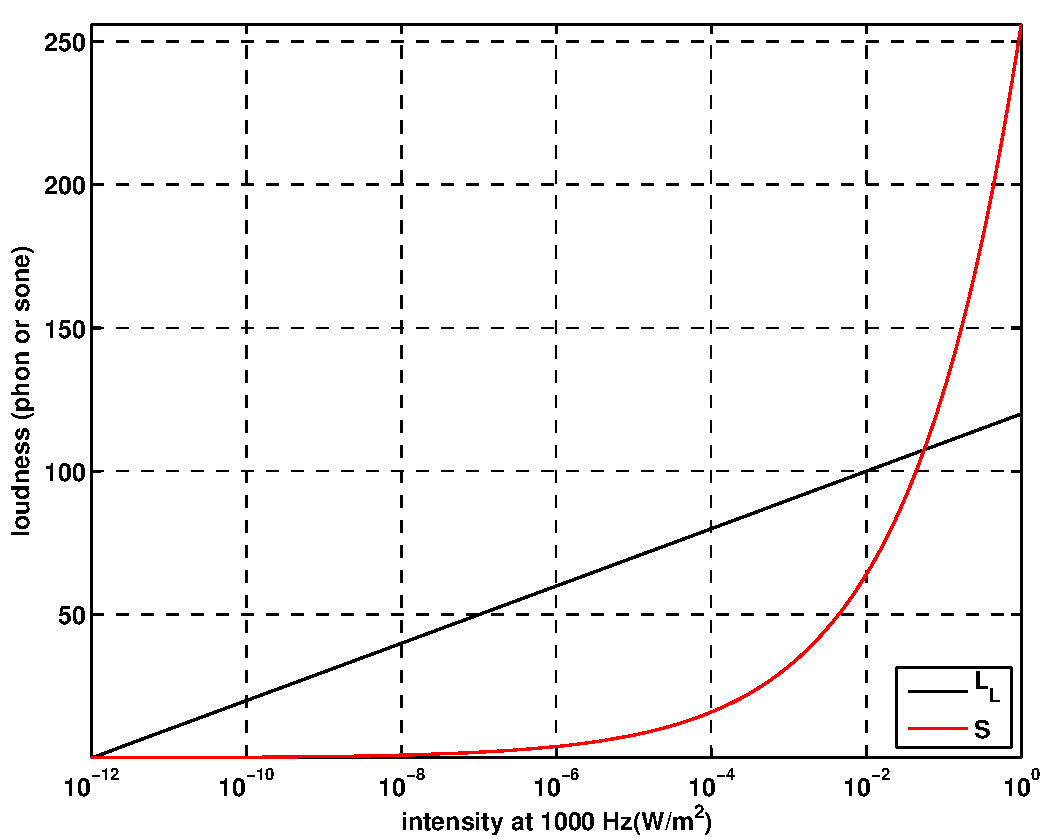
\includegraphics[width=.6\textwidth]{loudness-semilog}
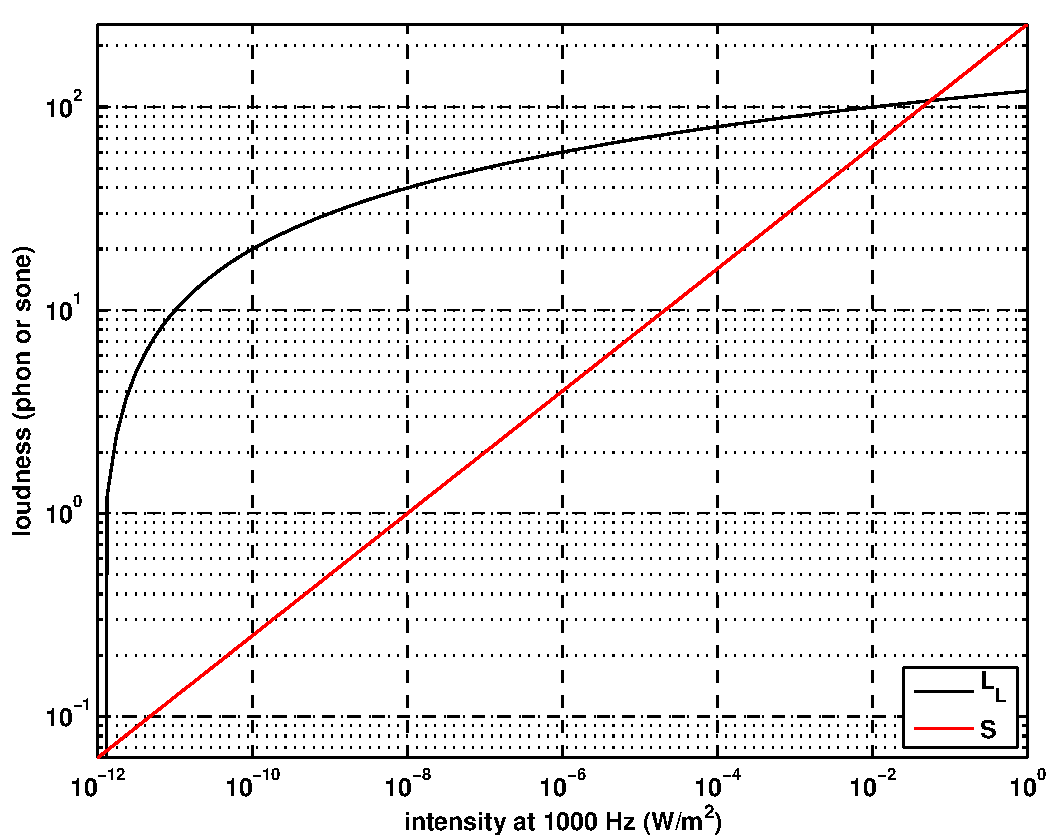
\includegraphics[width=.6\textwidth]{loudness-loglog}
\caption{Plots of $L_L$ and $S$ versus intensity $I$ 
for a pure tone with frequency 1000~Hz.
Top panel: $L_L$ and $S$ plotted on a linear vertical scale.
Bottom panel: $L_L$ and $S$ plotted on a logarithmic scale.
For both plots $I$ is plotted on a logarithmic vertical scale.}
\label{f:loudness}
\end{center}
\end{figure}
%

\i For example, 
from the top panel of Figure~\ref{f:loudness},
one sees that $L_L$ increases by 20~phon for 
each factor of 100 increase in $I$ (or 10~phon
for each factor of 10 increase in $I$).
From the bottom panel, one sees that $S$ increases
by a factor of 4 for each factor of 100 increase in $I$
(or a factor of 2 for each factor of 10 increase in $I$).

\ei

%%%%%%%%%%%%%%%%%%%%%%%%%%%%%%%%%%%%%%%%%%
\subsection{Sound from multiple sources}
\bi

\i Consider two instruments playing a note 
at the same time.
The sound waves from each instrument combine
with one another to produce a resultant wave 
with amplitude $p_{\rm tot}$ that can have 
any value between $p_1+p_2$ and $|p_1-p_2|$, 
where 
$p_1$, $p_2$ are the pressure amplitudes for
the two component waves.

\i One average, the resultant amplitude will 
have a value
%
\be
p_{\rm tot} = \sqrt{p_1^2 + p_2^2}
\ee
%
This is called an {\em incoherent} superposition
of two waves.

\i Since intensity is proportional to the
square of the pressure amplitude, it follows that the
intensity of the incoherent sum of the two sound waves
is given, on average, by
%
\be
I_{\rm tot} = I_1+I_2
\ee
%
Thus, intensities add.

\i Hence, 2 violins playing simultaneously produce
an intensity $2\times$ greater than that of a single
violin; 10 violins playing simultaneously produce
an intensity $10\times$ greater.
The corresponding increase in the sound intensity 
level $L_I$ (or the sound pressure level $L_p$) will be
%
\begin{align}
&10\log 2 \approx 3~{\rm dB}\quad({\rm two\ violins})
\\
&10\log 10 = 10~{\rm dB}\quad({\rm ten\ violins})
\end{align}
%

\i Note that to double the subjective loudness level $S$ 
requires $L_L$ to increase by 10~phon 
(or $L_p\approx L_I$ to increase by 10~dB at 1000~Hz).
This corresponds to a $10\times$ increase in the intensity $I$ 
of the sound at 1000~Hz.
{\em Hence, we would need 10~violins playing 
simultaneously to sound twice as loud as a single violin.}

\i Figure~\ref{f:multiplesources} shows the dependence
of the pressure difference $p$, intensity $I$,
sound loudness level $L_L$, and subjective loudness level
$S$ as a function of the number of sources $N$ ranging
from 1 to 100.
We are assuming here that the sources are producing
indentical pure tones that add incoherently.
%
\begin{figure}[htbp]
\begin{center}
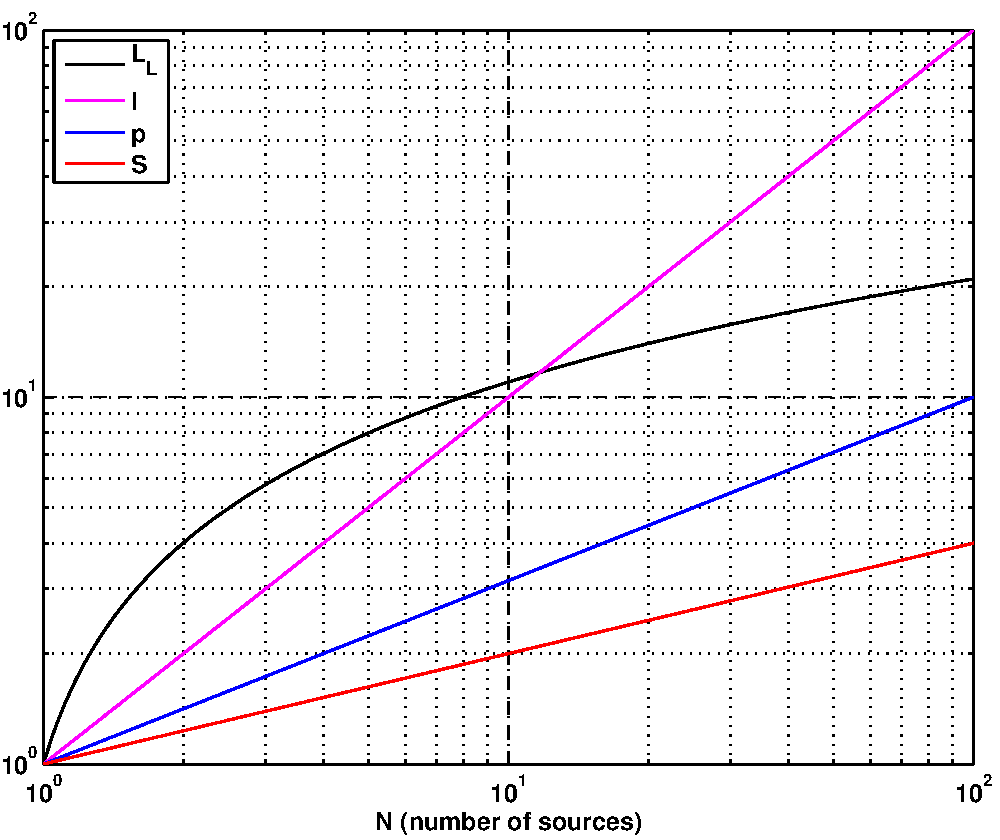
\includegraphics[width=.6\textwidth]{multiplesources}
\caption{Plots of total $p$, $I$, $L_L$, and $S$ 
versus the number of identical incoherent sources $N$.}
\label{f:multiplesources}
\end{center}
\end{figure}
%

\i Note that $I$ increases linearly with the number of
sources $N$, $p$ increases like $\sqrt{N}$ and 
$S$ like $N^{\log 2}$, all compared to their values 
for a single source ($N=1$).
The sound loudness level $L_L$ (which equals the sound
pressure level $L_p$ or the sound intensity level $L_I$
at $f=1000~{\rm Hz}$) increases by 10~dB for each factor
of 10 increase in the number of sources.

\ei

%%%%%%%%%%%%%%%%%%%%%%%%%%%%%%%%%%%%%%%%%%%%%%%
\subsection{Complex tones and masking}
\bi

\i A complex tone is made of two or more frequencies.

\i Loudness of complex tones is more complicated than
for pure tones.
For example, broadband sounds (like white noise) are perceived
to be louder than equally intense pure tones.

\i A summary of the key findings is given below:

(i) If the frequency components of a sound lie 
within a 
critical bandwidth (roughly one-third of an octave 
around a center frequency), then intensities
add just like for pure tones described above,
and subjective loudness $S$ is calculated
from the sound loudness level $L_L$ as before.
 
(ii) If the frequency components extend beyond
a critical bandwidth, then the perceived loudness
is greater than that for pure tones, approaching
the sum $S_{\rm tot} = S_1+S_2+\cdots$.

(iii) If the frequency components are widely
separated, the listener tends to focus on just 
a single component and assigns a total loudness 
equal to that of the single component.

\i Masking occurs when one tone dominates another
to such an extent that one doesn't hear the other
tone:

(i) If the two tones are widely separated in frequency
little masking occurs. 

(ii) Low-frequency tones more easily masks high-frequency
tones than vice-versa.

\i These statements can be understood in terms of the 
excitations of the basilar membrane produced
by pure tones.
The excitations are asymmetrical with a long
tail that extends toward the high-frequency end
of the membrane as shown in Figure~\ref{f:asymmetry_masking}.
%
\begin{figure}[htbp]
\begin{center}
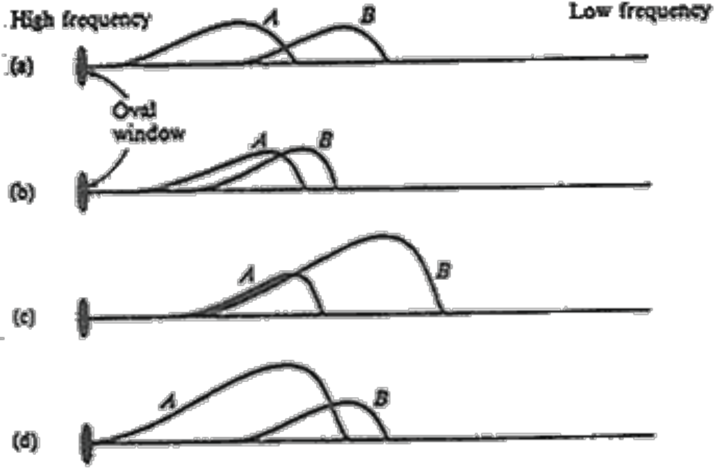
\includegraphics[width=.8\textwidth]{asymmetry_masking}
\caption{Excitations of the basilar membrane
corresponding to two pure tones $A$ (high frequency)
and $B$ (low frequency).
(a) Two equally-intense tones that barely overlap.
(b) Two equally-intense tones that significantly overlap.
(c) A more intense low-frequency tone that completely
masks a less intense high-frequency tone .
(d) A more intense high-frequency tone that only partially
masks a less intense low-frequency tone.
(From ``Science of Sound," by Rossing, Moore, and Wheeler.)}
\label{f:asymmetry_masking}
\end{center}
\end{figure}
%

\ei

%%%%%%%%%%%%%%%%%%%%%%%%%%%%%%%%%%%%%%%%%%%%%%%
\subsection{Pitch}
\bi

\i Just noticeable difference (JND):
the minimum difference in the frequencies of 
two pure tones played sequentially that can
be distinguished from one another.

\i The JND is approximately 0.5~\% of the 
center frequency, corresponding to roughly 
1/10th of a semitone or 10 cents.
For example, at A4 (440~Hz) the JND is 
approximately 2.2~Hz.

\i The JND has the same general dependence on 
frequency as does the critical bandwidth 
for the cochlea, but the JND is about a factor 
of 30 times smaller than the critical bandwidth.
(Recall: The critical bandwidth is about 
25\% of the center frequency, corresponding
to 1/3 of an octave, or 4 semitones.
For example, at A4 (440~Hz) the critical bandwidth
is approximately 110~Hz.

\i Limit of frequency resolution:
the minimum difference between two pure tones 
played simultaneously that can be distinguished
from one antother.

\i The limit of frequency resolution is about
$10\%$ of the center frequency, corresponding
to about 2 semitones.

\i Analogy: The sense of touch on the skin of 
your forearm using two pencil erasers.  
The separation of the erasers corresponds to the
JND or the limit of frequency resolution depending
on whether the touches are done sequentially or at 
the same time.

\i \demo 
Do the pencil eraser experiment.

\i Perfect (or absolute) pitch:
Ability to determine the absolute pitch 
of a tone without regard to a reference tone.

Only about 0.01\% of the population has
perfect pitch (so 1 out of 10000 people). 

\i There is controversy regarding it's origin.
Possible theories:
(i) hereditary,
(ii) can be acquired through training, 
(iii) everyone initially has perfect pitch, 
but it is lost without training,
(iv) all children could be taught to have
absolute pitch if it is done at the right
stage in their development (imprinting).

\i Missing fundamental, subjective fundamental, 
or periodicity pitch:

\i \ex
A complex tone consisting of harmonics
200~Hz, 300~Hz, 400~Hz, etc., will be heard
as having a pitch with a fundamental frequency of 100~Hz.

\i \ex
A complex tone consisting of the odd harmonics
300~Hz, 500~Hz, 700~Hz, etc., will also be heard
as having a pitch with a fundamental frequency of 100~Hz.

\i The missing fundamental doesn't exist as a 
physical sound wave; 
exists in central nervous system.

\i Combination tones: 
(sum and difference tones)
due to non-linear response of the human ear to 
an incident sound wave.

\i Asymmetries in the response of the 
human ear cause a pure tone to be represented
by a distorted wave with harmonics of the original wave.
These are called {\em aural harmonics}.

\i Combination tones exist as physical waves.
Difference tones are stronger than sum tones.
The effect is greatest when the two tones are
intense.

\i \ex
Play two notes simultaneously on a piano 
a fifth apart, e.g., C4 and G4.
The frequencies differ by a factor of 3/2.
If the two notes are played sufficiently loudly,
one hears the difference tone C3, which is an octave 
below C4.

\i Ohm's law of hearing:

One can only hear a pitch corresponding to 
a particular frequency if there is power at
that frequency.

Our perception of a sound depends only on
the spectrum of its partials, and 
not on the phase relationship of the partial waves.

\i Place theory of pitch:
frequency domain

\i Periodicity theory of pitch:
time domain

\i Both have some validity.

\i \ex
Consider a 200~Hz amplitude modulation of a 1200~Hz
carrier wave.
The result of the modulation is a linear superposition 
of sine waves having frequencies 1000~Hz, 1200~Hz, 1400~Hz.

The ear hears a pitch of 200~Hz, which corresponding 
to the difference tone the 1000~Hz and 1200~Hz components.
This pitch can also be thought of as the {\em missing fundamental} 
of a harmonic series with fundamental frequency $f_1=200~{\rm Hz}$.
The frequencies 1000~Hz, 1200~Hz, and 1400~Hz correspond
to the 5th, 6th, and 7th harmonics.

\i \ex
Now consider
a 200~Hz amplitude modulation of a 1240~Hz
carrier wave.
The result of the modulation is a linear superposition 
of sine waves having frequencies 1040~Hz, 1240~Hz, 1440~Hz.

Although there is still a difference frequency of 200~Hz,
the ear now hears a pitch of about 207~Hz.
This can be thought of as the missing fundamental of a
harmonic series with fundamental frequency $f_1=207~{\rm Hz}$.
The frequencies 1040~Hz, 1240~Hz, and 1440~Hz are
approximately equal to the 5th, 6th, and 7th harmonics 
of 207~Hz (1035~Hz, 1242~Hz, and 1449~Hz).

\ei

